\section{ĐỀ SỐ \thesection } %DỀ 13 QUẬN 6
\setcounter{bt}{0}

%%Câu 1.
\begin{bt} Thực hiện các phép tính
	\begin{listEX}[2]
		\item $345 + (-120) + (-275) + 400$;
		\item $3^{4} \cdot 3^{2} : 3^{5} - \left\{2 \cdot \left[50 - \left(12 - 2^{2} \cdot 3\right)\right]\right\}$.
	\end{listEX}
	\loigiai{a) $350$ \hfill b) $-97$.
	}
\end{bt}


%%Câu 2.
\begin{bt}Tìm  $x$ biết:
	\begin{listEX}[2]
		\item $25 + 4 \cdot x = 81$
		\item  $3^{2x} - 27 = 54$
	\end{listEX}
	\loigiai{a) $x=14$ \hfill b) $x=2$.
	}
\end{bt}



%%Câu 3.
\begin{bt}
	 	Hình dưới đây mô tả cửa xếp tự động. Mỗi khung như hình 3.1 được nối bởi các thanh inox có dạng hình thoi cạnh 30 cm.
	 \begin{center}
	 	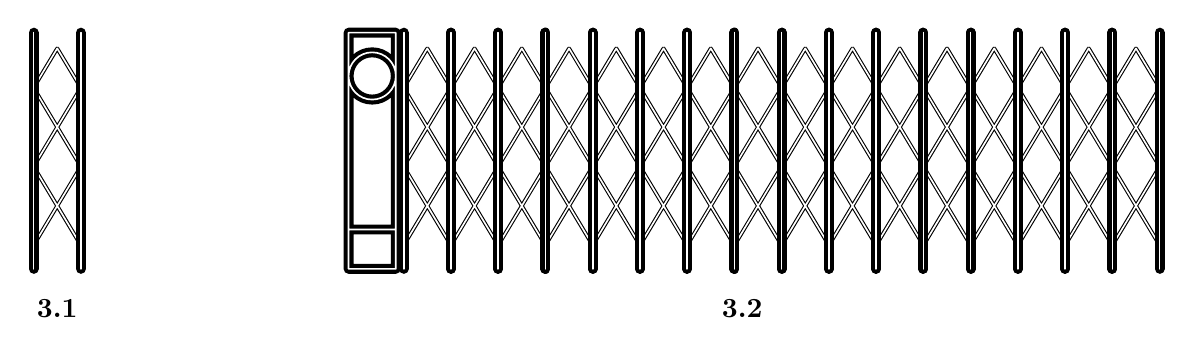
\begin{tikzpicture}[line cap=round,line join=round]
	 		% Define the basic properties
	 		\def\postheight{3}
	 		\def\postwidth{0.2}
	 		\def\crosslength{0.5}
	 		\def\gap{0.6}
	 		\def\sections{8}
	 		
	 		% Draw the closed gate (3.1)
	 		\begin{scope}[shift={(0,0)}]
	 			\draw[double] (0,0.3) -- (\gap,1.3) (0,1.3) -- (\gap, 2.3) (0,2.3) -- (\gap/2,2.8)
	 			(0,1.3) -- (\gap,0.3) (0,2.3) -- (\gap, 1.3) (\gap/2,2.8) -- (\gap,2.3);
	 			\draw[double,line width=1.5pt] (0,0) -- (0,\postheight) (\gap,0) -- (\gap,\postheight);
	 		\end{scope}
	 		
	 		% Draw the open gate (3.2)
	 		\begin{scope}[shift={(4,0)}]
	 			\draw[double,line width=1.5pt] (0,0) rectangle (\gap,\postheight)
	 			(0,0) rectangle (\gap,0.5) (0,\postheight-0.5) rectangle  (0,\postheight-0.5-\gap)
	 			(\gap/2,\postheight-0.25-\gap/2) circle (\gap/2);
	 			% Draw the open sections of the gate
	 			\foreach \i in {1,2,...,16} {
	 				\begin{scope}[shift={(\i*\gap+0.1,0)}]
	 					\draw[double] (0,0.3) -- (\gap,1.3) (0,1.3) -- (\gap, 2.3) (0,2.3) -- (\gap/2,2.8)
	 					(0,1.3) -- (\gap,0.3) (0,2.3) -- (\gap, 1.3) (\gap/2,2.8) -- (\gap,2.3);
	 					\draw[double,line width=1.5pt] (0,0) -- (0,\postheight) (\gap,0) -- (\gap,\postheight);
	 				\end{scope}
	 			}
	 		\end{scope}
	 		
	 		% Add labels below each part
	 		\node at (0.3,-0.5) {\textbf{3.1}};
	 		\node at (9,-0.5) {\textbf{3.2}};
	 	\end{tikzpicture}
	 \end{center}
	 \begin{enumerate}
	 \item  Hỏi mỗi khung như hình 3.1 cần bao nhiêu mét thanh inox để nối?
	 \item Hỏi cửa xếp tự động ở hình 3.2 cần bao nhiêu mét thanh inox để nối?
	 \end{enumerate}
	\loigiai{a) $3$ m \hfill b) $48$ m.
	}
\end{bt}


%%Câu 4.
\begin{bt} Một nhà máy sản xuất có ba loại sản phẩm: sản phẩm A, sản phẩm B và sản phẩm C. Số lượng mỗi loại sản phẩm là:
	\begin{multicols}{3}
		\begin{itemize}
			\item Sản phẩm A: 48 cái.
			\item Sản phẩm B: 72 cái.
			\item Sản phẩm C: 108 cái.
		\end{itemize}
	\end{multicols}
	
	Nhà máy muốn đóng gói tất cả sản phẩm vào các thùng sao cho mỗi thùng chứa số sản phẩm bằng nhau mà không để thừa sản phẩm. Hỏi mỗi thùng sẽ chứa bao nhiêu sản phẩm và nhà máy có thể đóng được tối đa bao nhiêu thùng?
	\loigiai{Mỗi thùng sẽ chứa: $19$ sản phẩm. Và nhà máy có thể đóng được tối đa $12$ thùng.}
\end{bt}



%%Câu 5.
\begin{bt} 
	Một gian phòng có nền hình chữ nhật với kích thước là $3,6 \mathrm{~m}$ và $5,8 \mathrm{~m}$, có một cửa sổ hình chữ nhật kích thước là $0,8 \mathrm{~m}$ và $1,2 \mathrm{~m}$ và một cửa ra vào hình chữ nhật kích thước $1,2 \mathrm{~m}$ và 2 m . Tỉ lệ phần trăm diện tích các cửa so với diện tích nền nhà.
	\loigiai{Tỉ lệ phần trăm diện tích các cửa và diện tích nền nhà là $\frac{3,36}{20,88} \approx 16 \%$.
	}
\end{bt}


%%Câu 6.
\begin{bt} 
	Biểu đồ cột kép ở hình vẽ biểu diễn số lượng ca nhiễm SAR-COVID-2 và số lượng người tử vong (tính đến ngày $3 / 7 / 2021$ tại Việt Nam). Hỏi tỉ lệ tử vong vì SAR-COVID-2 ở tỉnh nào là cao nhất? Cho các tỉ lệ đó là bao nhiêu.
	\begin{center}
	\begin{tikzpicture}[scale=0.07,font=\small,line join=round,>=stealth]
		% --- Thông số ---
		\def\hoanh{100} 
		\def\tung{150}   % chiều cao trục tung đủ lớn để chứa cột 174
		\def\sc{5}       % hệ số tỉ lệ, chia giá trị thực để vừa trang
		\def\w{5}        % bề rộng mỗi cột
		
		% --- Trục toạ độ ---
		\draw[->] (0,0)node[left]{0}--(\hoanh,0) node[right,below]{\footnotesize \textbf{Tỉnh}};
		\draw[->] (0,0)--(0,\tung/\sc+10) node[above]{\footnotesize \textbf{Số lượng (Người)}};
		
		% --- Chia vạch tung ---
		\foreach \y in {50,100,...,200}{
			\draw (-0.15,\y/\sc) node[left]{$\y$} -- ++(0:0.3);
		}
		
		% --- Cột dữ liệu ---
		\foreach \x/\nhiem/\chet in {10/126/10,30/113/7,50/56/12,70/174/23}{
			% Nhiễm (kẻ xéo)
			\fill[pattern=north east lines,pattern color=blue!80!black,draw=blue!80!black]
			(\x-\w,0) rectangle ++(\w,\nhiem/\sc);
			\node[black,font=\footnotesize,anchor=south,yshift=1pt]
			at (\x-\w/2,\nhiem/\sc) {\nhiem};
			
			% Chết (chấm bi)
			\fill[pattern=dots,pattern color=red!80!black,draw=red!70!black]
			(\x,0) rectangle ++(\w,\chet/\sc);
			\node[black,font=\footnotesize,anchor=south,yshift=1pt]
			at (\x+\w/2,\chet/\sc) {\chet};
		}
		
		% --- Nhãn tên các tỉnh ---
		\foreach \x/\p in {15/Hưng~Yên,35/Nghệ~An,55/Đồng~Tháp,75/Phú~Yên}{
			\node[font=\footnotesize,rotate=15,anchor=north east] at (\x,-0.5){\textbf{\p}};
		}
		
		\fill[pattern=north east lines,pattern color=blue!80!black,draw=blue!80!black]
		(84,38) rectangle (87,35);
		\node[font=\footnotesize,anchor=west] at (87.2,35) {Nhiễm};
		
		\fill[pattern=dots,pattern color=red!80!black,draw=red!70!black]
		(84,42) rectangle (87,39);
		\node[font=\footnotesize,anchor=west] at (87.2,40.5) {Chết};
		
	\end{tikzpicture}	\vspace{0.1 em}
	{\footnotesize\itshape (Nguồn: https://vnexpress.net/)}
	\end{center}
	
	

	
	
	
	\loigiai{
			Tỉ lệ tử vong vì SAR-COVID-2 ở tỉnh Hưng Yên là $\frac{10}{126} \approx 7,94 \%$.\\
			 Tỉ lệ tử vong vì SAR-COVID-2 ở tỉnh Nghệ An là $\frac{7}{113} \approx 6,19 \%$.\\
			Tỉ lệ tử vong vì SAR-COVID-2 ở tỉnh Đồng Tháp là $\frac{12}{56} \approx 21,43 \%$.\\
			Tỉ lệ tử vong vì SAR-COVID-2 ở tỉnh Phú Yên là $\frac{23}{174} \approx 13,22 \%$.\\
			Vậy tỉ lệ tử vong vì SAR-COVID-2 ở tỉnh Đồng Tháp là cao nhất
	}
\end{bt}


